\chapter{Object-Oriented Design}
\label{chap:object_oriented_design}

\begin{figure}[ht]
	\hfill
	\begin{minipage}{0.5\textwidth}
		\centering
		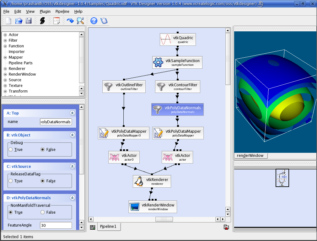
\includegraphics{VTKTextbook-10}\\
		\caption*{\texttt{VTK Designer image courtesy of vcreatelogic.com.}}
	\end{minipage}
\end{figure}

\firstletter{O}bject-oriented systems are becoming widespread in
the computer industry for good reason. \\Object-oriented systems are more modular, easier to maintain, and easier to describe than traditional procedural systems. Since the Visualization Toolkit has been designed and implemented using object-oriented design, we devote this chapter to summarizing the concepts and practice of object-oriented design and implementation.

\section{Introduction}
Today’s software systems try to solve complex, real-world problems. A rigorous software design and implementation methodology can ease the burden of this complexity. Without such a methodology, software developers can find it difficult to meet a system’s specifications. Furthermore, as specifications change and grow, a software system that does not have a solid, underlying architecture and design will have difficulty adapting to these expanding requirements.

\section{Bibliographic Notes}
There are several excellent textbooks on object-oriented design.
Both \cite{Rumbaugh91} and \cite{Birtwistle79} present language-independent design methodologies.
Both books emphasize modelling and diagramming as key aspects of design.
\cite{Meyer88} also describes the OO design process in the context of Eiffel, an OO language.
Another popular book has been authored by Booch \cite{Booch91}.

Anyone who wants to be a serious user of object-oriented design and implementation should read the books on Smalltalk \cite{Goldberg83} \cite{Goldberg84} by the developers of Smalltalk at Xerox Parc.
In another early object-oriented programming book, \cite{Cox86} describes OO techniques and the programming language Objective-C.
Objective-C is a mix of C and Smalltalk and was used by Next Computer in the implementation of their operating system and user interface.

There are many texts on object-oriented languages. CLOS \cite{Keene89} describes the Common List Object System. Eiffel, a strongly typed OO language is described by \cite{Meyer88} .
Objective-C \cite{Cox86} is a weakly typed language.

Since C++ has become a popular programming language, there now many class libraries available for use in applications.
\cite{Gorlen90} describes an extensive class library for collections and arrays modeled after the Smalltalk classes described in \cite{Goldberg83} .
\cite{Stepanov94} and \cite{Musser94} describe the Standard Template Library, a framework of data structures and algorithms that is now a part of the ANSI C++ standard. Open Inventor \cite{Inventor} is a C++ library supporting interactive 3D computer graphics.
The Insight Segmentation and Registration Toolkit (ITK) is a relatively newclass library often used in combination with VTK \cite{ITK} for medical data processing. VXL is a C++library for computer vision research and implementation \cite{VXL}.
Several mathematical libraries such as VNL (a part of VXL) and Blitz++ \cite{Blitz} are also available. A wide variety of other C++ toolkits are available, Google searches \cite{Google} are the best way to find them.

C++ texts abound. The original description by the author of C++ \cite{Stroustrup84} is a must for any serious C++ programmer. Another book \cite{Ellis90} describes standard extensions to the language.
These days the UML book series—of which \cite{Booch98} and \cite{Rumbaugh98} are quite popular—are highly recommended resources. Several books on generic programming \cite{Austern99} and STL \cite{Musser96} are also useful. Check with your colleagues for their favourite C++ book.
To keep in touch with new developments there are conferences, journals, and Web sites. The strongest technical conference on object-oriented topics is the annual Object-Oriented Programming Systems, Languages, and Applications ( OOPSLA ) conference. This is where researchers in the field describe, teach and debate the latest techniques in object-oriented technology. The bimonthly Journal of Object-Oriented Programming (JOOP) published by SIGS Publications, NY, presents technical papers, columns, and tutorials on the field. Resources on the World Wide Web include the Usenet newsgroups comp.object and comp.lang.c++.

\printbibliography